\begin{figure}
\captionsetup[subfigure]{justification=centering}
\begin{subfigure}[t]{0.48\textwidth}
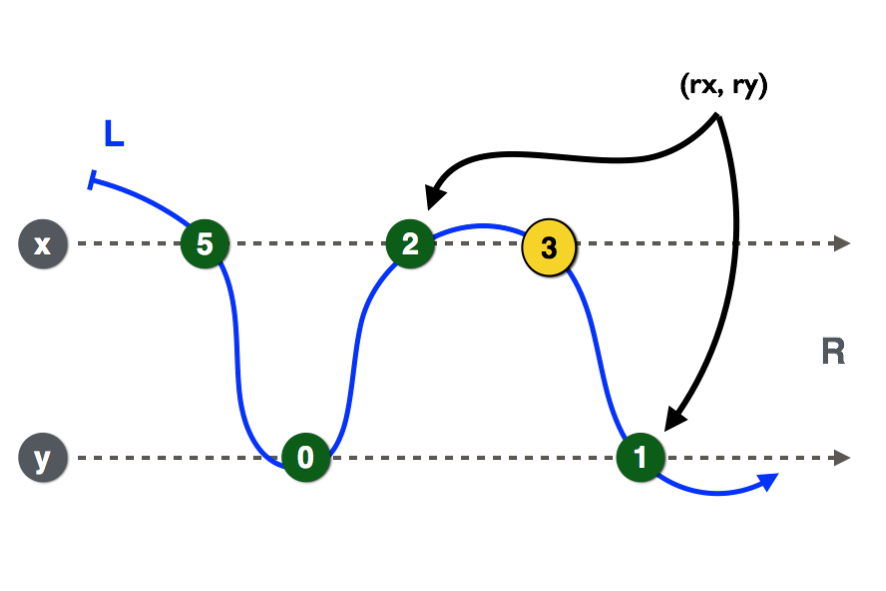
\includegraphics[height=4cm]{res/relink-before2.pdf}
\caption{\label{fig:reorder:before}} % Logical $=$ Real Time order, not a snapshot}
\end{subfigure} \hfill
\begin{subfigure}[t]{0.48\textwidth}
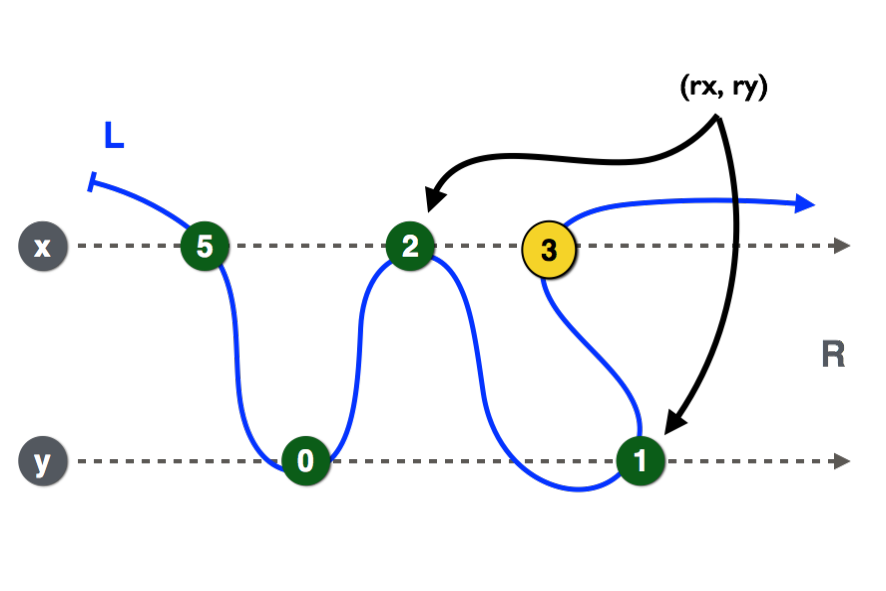
\includegraphics[height=4cm]{res/relink-after2.pdf}
\caption{\label{fig:reorder:after}} % Logical $\neq$ Real Time order, snapshot OK}
\end{subfigure}%
%
\caption{\label{fig:reorder} Changing the logical ordering (solid line $L$) of write
  events from (5, 0, 2, 3, 1) in (\subref{fig:reorder:before}) to (5,
  0, 2, 1, 3) in (\subref{fig:reorder:after}), to reconcile with {\tt
    scan} returning the snapshot $\x=2, \y=1$, upon missing the write
  of $3$. Dashed lines $R$ represent real-time ordering.}
\end{figure}
